\section{Przeglądanie zleceń przez klientów}

Klienci muszą posiadać możliwość przeglądania utworzonych przez siebie zleceń. Ekran, który taką funkcjonalność zapewnia, został przedstawiony na rysunku \ref{fig:client-jobs}. Zawiera on listę zleceń, którą można ograniczyć do konkretnych usług przy pomocy mechanizmu filtrowania.
%  Lista jest posortowana chronologicznie, najnowsze zlecenia znajdują się na jej szczycie.
Elementy listy zawierają ikonkę pinezki, której kolor zdradza, czy dane zlecenie jest jeszcze otwarte i czy wykonawcy mogą się dalej zgłaszać. Jeśli tak jest, to ma ona kolor zielony, a w przeciwnym wypadku kolor czerwony. Jeżeli miały miejsce jakieś zdarzenia dotyczące zlecenia, które nie zostały jeszcze odczytane, to wewnątrz elementu listy wyświetlana jest taka informacja. 
%Wybranie z listy któregoś ze zleceń spowoduje przejście do ekranu zgłoszonych ofert. Opisano go w kolejnej sekcji.

\begin{figure}[ht!]
  \centering
    \fbox{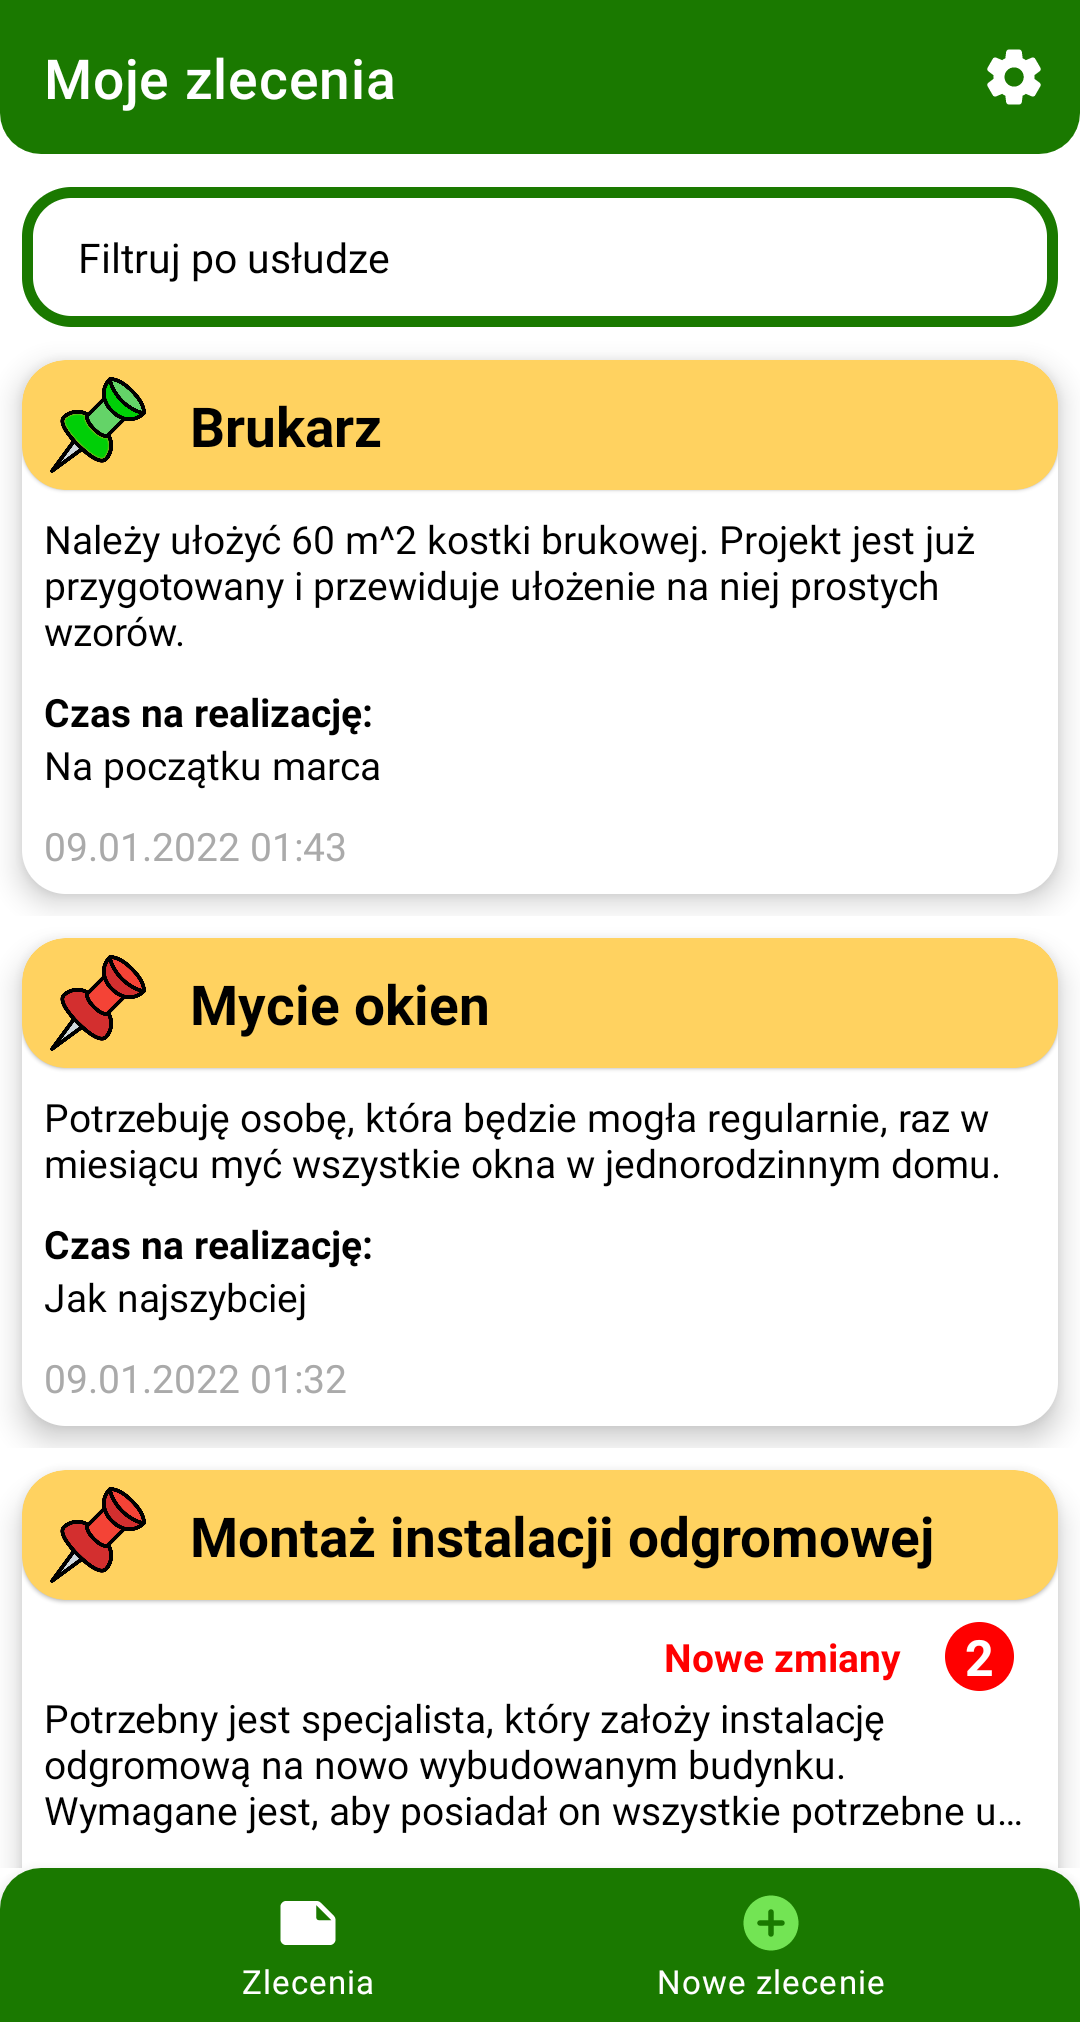
\includegraphics[width=0.33\linewidth]{screens/client_jobs.png}}
  \caption{Ekran listy utworzonych przez klienta zleceń}
  \label{fig:client-jobs}
\end{figure}
